\documentclass[a4paper]{article}
\usepackage[bottom=10em]{geometry}

\usepackage[T1]{fontenc}	
\usepackage{amsmath}
\usepackage{amssymb}
\usepackage{graphicx}
\usepackage{fancyhdr}
\usepackage{array}
\usepackage{float}
\usepackage{booktabs}

\pagestyle{fancy}
\lhead{Computer Excercise 2}
\rhead{Kristoffer Nordström \& Noah Hansson}

\title{Computer Exercise 2 - NEKN83}
\author{Kristoffer Nordström \& Noah Hansson}
\date{\today}

\setlength{\parskip}{0.7em}
\setlength{\parindent}{0pt}
\setlength{\floatsep}{6pt plus 1.0pt minus 2.0pt}
\setlength{\textfloatsep}{10pt plus 1.0pt minus 2.0pt}

\begin{document}

\maketitle


\section{Introduction}
In this computer exercise the aim is to implement ways to implement and evaluate Expected Shortfall\footnote{Henceforth referred to as ES} for the US stock market index SP500. Different methods of estimating ES will be compared and discussed in the conclusion.

\section{Method}
The data used for this exercise is the daily recorded returns of the SP500 market index during the years 2013 - 2015. The returns are then converted to losses by assuming that we hold a portfolio of \$1000 each day. We will then use this data to evaluate Value-at-Risk\footnote{Henceforth referred to as VaR}, and then the ES, using different assumptions and implementations. The ES will be tested using the Acerbi \& Szekely Z-test statistic. The VaR and ES will estimated in five different ways:
\begin{itemize}
    \item Normal
    \item Normal-EWMA
    \item T-dist
    \item T-dist EWMA
    \item Basic Historical Simulation
\end{itemize}
Through the whole computer exercise the certainty level for VaR and ES will be 97.5\%. Finally, we implement a Basel-type traffic light system for underestimation to classify the different estimation methods.

All data and calculations are handled in Microsoft Excel, and the plots are generated in Python.

\section{Results}


\begin{table}[H]
    \centering
    \caption{The different models and Z-tests}
    \vspace{0.2cm}
    \begin{tabular}{lrrr}
        \toprule
                Model &  Z (test stat.) & Accept/Reject & Result ES traffic light system \\
        \midrule
                ES-N &       -1.742215 &        Reject &                         Yellow \\
            ES\_N\_EWMA &       -0.727824 &        Reject &                         Yellow \\
                ES-t &       -1.203534 &        Reject &                         Yellow \\
            ES-t-EWMA &       -0.628559 &        Accept &                          Green \\
            ES-BHS &       -1.000707 &        Reject &                         Yellow \\
        \bottomrule
    \end{tabular} 
\end{table}



\begin{table}[H]
    \centering
    \caption{The different models and number of VaR violations}
    \vspace{0.2cm}
    \begin{tabular}{lrr}
        \toprule
              Model &  Number over VaR & Results VaR traffic light system \\
        \midrule
              VaR-N &               14 &                           Yellow \\
         VaR-N-EWMA &                9 &                            Green \\
              VaR-t &               11 &                           Yellow \\
         VaR-t-EWMA &                9 &                            Green \\
            VaR-BHS &               11 &                           Yellow \\
        \bottomrule
    \end{tabular}    
\end{table}
 
\begin{figure}[H]
    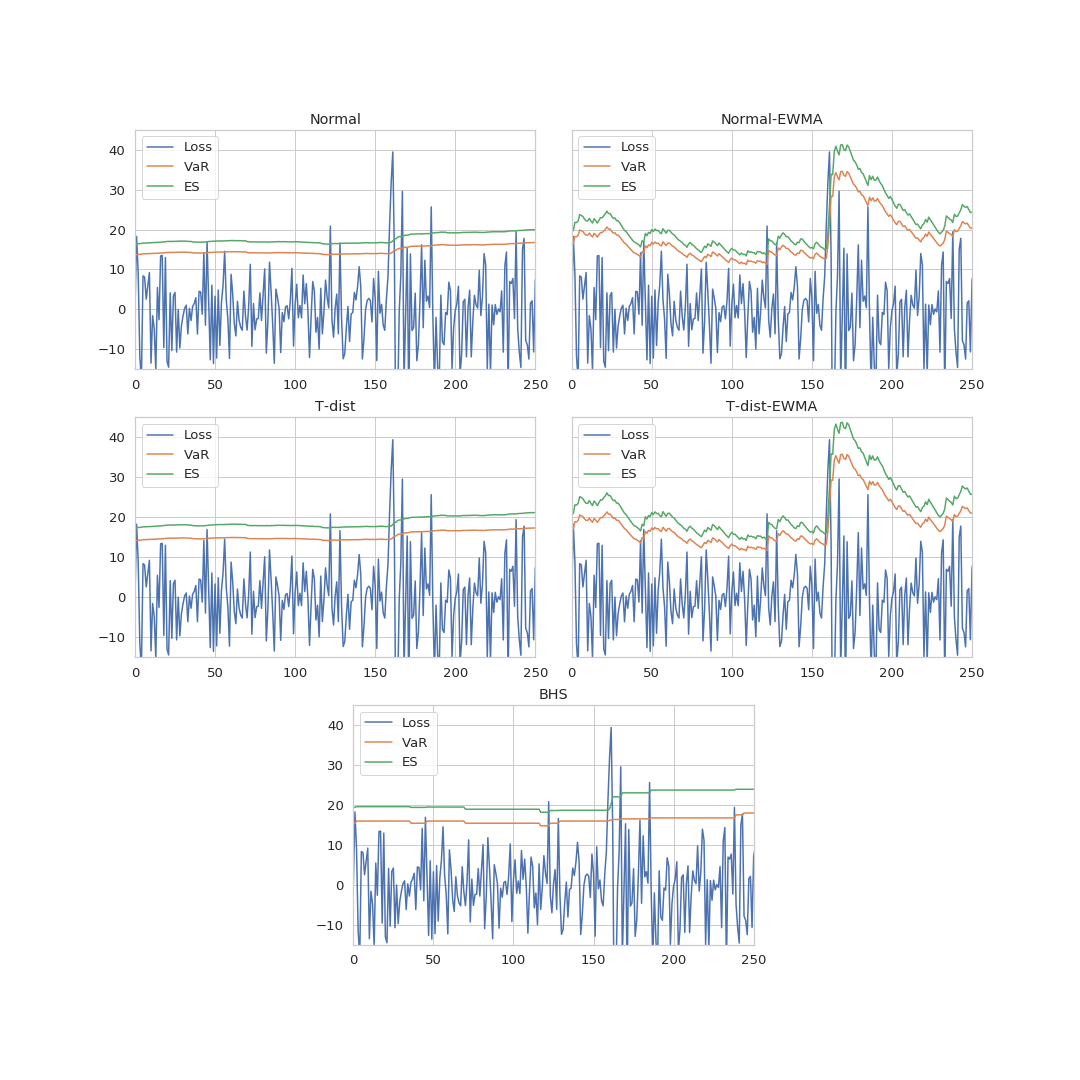
\includegraphics[width=\textwidth]{plot.png}
    \caption{Observed loss compared to $VaR_{99\%}$ estimates based on EWMA volatility predictions}
    \label{var2}
\end{figure}

\section{Conclusion}


\end{document}